\documentclass{article}

\usepackage[a4paper,margin=1in,landscape]{geometry}
\usepackage{amsmath}
\usepackage{graphicx}
\usepackage[misc]{ifsym}

\renewcommand{\labelitemi}{--}
\newcommand{\tgap}{\hspace{1pt}}
\newcommand{\gap}{\hspace{4pt}}

\makeatletter
\def\bbordermatrix#1{\begingroup \m@th
  \@tempdima 4.75\p@
  \setbox\z@\vbox{%
    \def\cr{\crcr\noalign{\kern2\p@\global\let\cr\endline}}%
    \ialign{$##$\hfil\kern2\p@\kern\@tempdima&\thinspace\hfil$##$\hfil
      &&\quad\hfil$##$\hfil\crcr
      \omit\strut\hfil\crcr\noalign{\kern-\baselineskip}%
      #1\crcr\omit\strut\cr}}%
  \setbox\tw@\vbox{\unvcopy\z@\global\setbox\@ne\lastbox}%
  \setbox\tw@\hbox{\unhbox\@ne\unskip\global\setbox\@ne\lastbox}%
  \setbox\tw@\hbox{$\kern\wd\@ne\kern-\@tempdima\left[\kern-\wd\@ne
    \global\setbox\@ne\vbox{\box\@ne\kern2\p@}%
    \vcenter{\kern-\ht\@ne\unvbox\z@\kern-\baselineskip}\,\right]$}%
  \null\;\vbox{\kern\ht\@ne\box\tw@}\endgroup}
\makeatother

\begin{document}

\section*{Slides}

If the two outcomes are \emph{not} mutually exclusive:

\[
P\left(\left\{2\times{H}\right\} \cup \left\{3\times{H}\right\}\right)
= \frac{4}{8} + \frac{1}{8} - \frac{1}{8} = \frac{4}{8} = 0.5
\]

\[
P\left(\left\{2\times{H}\right\} \cap \left\{1\times{T}\right\}\right) +
P\left(3 \times{H}\right)
\]

\begin{itemize}
\item the mean of $x$ is 9
\item the variance of $x$ is 11
\item the mean of $y$ is 7.50
\item the variance of $y$ is 4.125
\item the correlation coefficient of $x$ and $y$ is 0.816
\item the best fit line is given by $y = 3.00 + 0.500 x$
\end{itemize}

\begin{tabular}{r|cccccccccccccccccccc}
  urn: & 1 & 2 & 3 & 4 & 5 & 6 & 7 & 8 & 9 & 10 &
  11 & 12 & 13 & 14 & 15 & 16 & 17 & 18 & 19 & 20 \\
  10 samples selected with replacement: &
  5 & 2 & 12 & 19 & 10 & 5 & 3 & 19 & 11 & 4
  & & & & & & & & & & \\
  10 samples selected with replacement: &
  $\boxed{5}$ & 2 & 12 & $\boxed{19}$ & 10 & $\boxed{5}$ & 3 & $\boxed{19}$ & 11 & 4
  & & & & & & & & & & \\
  10 samples selected without replacement: &
  15 & 8 & 13 & 5 & 4 & 19 & 7 & 1 & 20 & 10
  & & & & & & & & & & 
\end{tabular}

\[
P(H,H,T) +
P\left(\raisebox{-2pt}{\Cube{2}},\raisebox{-2pt}{\Cube{6}}\right) -
P\left(H,H,H \cap \raisebox{-2pt}{\Cube{2}},\raisebox{-2pt}{\Cube{6}}\right)
\]

\[
p = 2/3
\]

We failed to reject $H_\circ$ for $\hat{p}=\frac{2}{5}=0.4$. How about
$\hat{p}=\frac{6}{15}=0.4$?

\[
k \in R
\]

Next, how about $\hat{p}=\frac{12}{30}=0.4$?

Which values of $p$ are compatible with the observation of $k=2$
successes out of $n=5$ claims?

\[
P({k}\leq{2}|p=2/3,n=5) =
\sum\limits_{i=0}^{2}\binom{5}{i}(2/3)^i(1/3)^{n-i} = 0.21 \geq \alpha/2
\]

Assuming that $H_\circ$ is true, the probability of incurring a type-I
error is:\\

1 experiment: $\alpha = 5\%$\\

2 experiments: $1-(1-\alpha)^2=9.75\%$\\

3 experiments: $1-(1-\alpha)^3=14\%$\\

48 experiments:   $1-(1-\alpha)^{48}=91.5\%$\\

$N$ experiments:   $1-(1-\alpha)^{N}\%$\\

Bonferroni correction: $\alpha/N$\\

What is $\lambda$?\\

\textbf{the binomial distribution}\\

\textbf{the Poisson distribution}\\

What is so normal about the Gaussian distribution?\\

What is $s[z]$?\\

\[
s[d] = \sqrt{s[x]^2 + s[y]^2}
\]

\[
z = x + y
\]

\[
z = x - y
\]

\[
s[z]^2 = s[x]^2 + s[y]^2
\]

\[
z = xy
\]

\[
\left(\frac{s[z]}{z}\right)^2 =
\left(\frac{s[x]}{x}\right)^2 + \left(\frac{s[y]}{y}\right)^2
\]

\[
s[y]^2 = y^2\left(2\frac{s[t]}{t}\right)^2
\]

\[
2 \times 0.0000042 = 0.0000084 < \alpha
\]

P($\geq{9.0}$ earthquake)?

\begin{center}
\begin{tabular}{c@{~}c@{~}c@{~}c@{~}c@{~}c@{~}c@{~}c@{~}c@{~}c@{~}c@{~}c@{~}c@{~}c@{~}c}
  44 & + 51 & + 79 & + 65 & + 27 & + 31 & + 4 & + 355 & +
  22 & + 352 & + 287 & + 7 & + 287 & + 339 & + 0 \\
  276 & + 342 & + 355 & + 334 & + 296 & + 7 & + 17 & +
  351 & + 349 & + 37 & + 339 & + 40 & + 324 & + 325 & + 334\\ \hline
  & & & & & & & 30 & & & & & & & 
\end{tabular}
\end{center}

\[
= 189.2^\circ
\]

\[
\sin[\theta\pm\phi] = \sin[\theta]\cos[\phi]\pm\cos[\theta]\sin[\phi]
\]

\[
359^\circ - 1^\circ = 2^\circ
\]

\[
\bar{R} = 0.88
\]

\[
s_c = 0.51
\]

\[
s_c = 2.04
\]

\begin{tabular}{c|cccccccccc}
x & 0.85 & 0.84 & 0.83 & 0.8 & 0.77 & 0.75 & 0.74 & 0.73 & 0.71 & 0.6 \\
y & 0.53 & 0.54 & 0.56 & 0.6 & 0.64 & 0.66 & 0.67 & 0.68 & 0.71 & 0.8 \\
\hline
x & -0.87 & -0.85 & -0.83 & -0.8 & -0.77 & -0.75 & -0.74 & -0.73 & -0.69 & -0.64 \\
y & -0.50 & -0.53 & -0.56 & -0.6 & -0.64 & -0.66 & -0.67 & -0.68 & -0.72 & -0.77 \\
\end{tabular}

\clearpage

\section*{Quizzes}

\begin{minipage}{\linewidth}
Given $k=9$ successes out of n=10 binomial trials, carry out a hypothesis test for\medskip

\( H_0: p=0.6\)\medskip

versus\medskip

\( H_a: p > 0.6\)\medskip

at a 95\% confidence level.\medskip

\begin{tabular}{r|ccccccccccc}
  $X$ & 0 & 1 & 2 & 3 & 4 & 5 & 6 & 7 & 8 & 9 & 10 \\
  $P(X)$ & 0.0001 & 0.0016 & 0.01062 & 0.0425 & 0.1115 & 0.2007 &
  0.2508 & 0.2150 & 0.1209 & 0.0403 & 0.0060 \\
  $P(x \leq X)$ & 0.0001 & 0.0017 & 0.01230 & 0.0548 & 0.1662 &
  0.3669 & 0.6177 & 0.8327 & 0.9536 & 0.9940 & 1 \\
  $P(x \geq X)$ & 1 & 0.9999 & 0.9983 & 0.9877 & 0.9452 &
  0.8338 & 0.6331 & 0.3823 & 0.1673 & 0.0464 & 0.0060
\end{tabular}\medskip

Can the null hypothesis be rejected?
\end{minipage}

\vspace{1cm}

\noindent\begin{minipage}{\linewidth}
Given $k=9$ successes out of n=10 binomial trials, carry out hypothesis test of\medskip

\( H_\circ: p=0.6\)\medskip

versus\medskip

\( H_a: p \neq 0.6\)\medskip

at a 95\% confidence level.\medskip

\begin{tabular}{r|ccccccccccc}
  $X$ & 0 & 1 & 2 & 3 & 4 & 5 & 6 & 7 & 8 & 9 & 10 \\
  $P(X)$ & 0.0001 & 0.0016 & 0.01062 & 0.0425 & 0.1115 & 0.2007 &
  0.2508 & 0.2150 & 0.1209 & 0.0403 & 0.0060 \\
  $P(x \leq X)$ & 0.0001 & 0.0017 & 0.01230 & 0.0548 & 0.1662 &
  0.3669 & 0.6177 & 0.8327 & 0.9536 & 0.9940 & 1 \\
  $P(x \geq X)$ & 1 & 0.9999 & 0.9983 & 0.9877 & 0.9452 &
  0.8338 & 0.6331 & 0.3823 & 0.1673 & 0.0464 & 0.0060
\end{tabular}\medskip

Can the null hypothesis be rejected?
\end{minipage}

\vspace{1cm}

\noindent\begin{minipage}{\linewidth}
Given $k=9$ successes out of n=10 trials, carry out a hypothesis test for\medskip

\( H_\circ: p=0.6\)\medskip

versus\medskip

\( H_a: p<0.6\)\medskip

at a 95\% confidence level?\medskip

\begin{tabular}{r|ccccccccccc}
  $X$ & 0 & 1 & 2 & 3 & 4 & 5 & 6 & 7 & 8 & 9 & 10 \\
  $P(X)$ & 0.0001 & 0.0016 & 0.01062 & 0.0425 & 0.1115 & 0.2007 &
  0.2508 & 0.2150 & 0.1209 & 0.0403 & 0.0060 \\
  $P(x \leq X)$ & 0.0001 & 0.0017 & 0.01230 & 0.0548 & 0.1662 &
  0.3669 & 0.6177 & 0.8327 & 0.9536 & 0.9940 & 1 \\
  $P(x \geq X)$ & 1 & 0.9999 & 0.9983 & 0.9877 & 0.9452 &
  0.8338 & 0.6331 & 0.3823 & 0.1673 & 0.0464 & 0.0060
\end{tabular}\medskip

Can the null hypothesis be rejected?
\end{minipage}

\vspace{1cm}

\noindent\begin{minipage}{\linewidth}

Here are some key quantiles (column names) of a binomial distribution\\
with \(n=100\) and parameter values \(p\) given as row names:\\

\( \begin{array}{c|cccccccccc}
  ~ & 0.01 & 0.025 & 0.05 & 0.1 & 0.5 & 0.9 & 0.95 & 0.975 & 0.99 \\ \hline
  0.466 & 35 & 37 & 38 & 40 & 47 & 53 & 55 & 56 & 58 \\
  0.497 & 38 & 40 & 42 & 43 & 50 & 56 & 58 & 60 & 61 \\
  0.513 & 40 & 42 & 43 & 45 & 51 & 58 & 59 & 61 & 63 \\
  0.682 & 57 & 59 & 60 & 62 & 68 & 74 & 76 & 77 & 79 \\
  0.697 & 59 & 60 & 62 & 64 & 70 & 76 & 77 & 78 & 80 \\
  0.724 & 62 & 63 & 65 & 67 & 72 & 78 & 80 & 81 & 82 \\
\end{array} \)\medskip

What  is the  95\%  confidence interval  for \(p\)  if  the number  of\\
successes is \(k=60\) out of \(n=100\)?

\vspace{1cm}

\end{minipage}

\begin{align*}
  \mbox{P(wrong decision)} = & 1 - \left(1 - \frac{1}{7\times{10}^7}\right)^{1\times{10}^7} \\
  = & 1 - \exp\!\left(1\times{10}^7 \ln\!\left(1 - \frac{1}{7\times{10}^7}\right)\right) \\
  = & 1 - \exp\!\left(-\frac{1\times{10}^7}{7\times{10}^7}\right) \\
  = & 1 - \exp(-1/7) = 0.13 \\
\end{align*}

\[
\frac{\mbox{P(double SIDS)}}{\mbox{P(double homicide)}} = \frac{21700 \times 123}{1300 \times 228} = \frac{9}{1}
\]

\vspace{1cm}

\noindent\begin{minipage}{\linewidth}

Consider the following two rock specimens:\medskip

\(
\begin{array}{ccccc}
  \mbox{specimen} & \mbox{mass (g)} & \sigma(\mbox{mass}) &
  \mbox{volume}(\mbox{cm}^3) & \sigma(\mbox{volume}) \\ \hline
  A & 105 & 2 & 36 & 0.15\\ B & 30 & 2.5 & 10 & 0.4
\end{array}
\)

\begin{enumerate}
\item Compute the densities of rocks \(A\) and \(B\).
\item Propagate their respective uncertainties.
\item Construct approximate 95\% confidence intervals for the two densities.
\item Is there a significant difference in density between samples \(A\) and \(B\)?
\end{enumerate}

\end{minipage}

\vspace{1cm}

\noindent\begin{minipage}{.55\linewidth}

Sand may contain a variety of minerals with different densities. For
example, zircon has a density of \(4.85\pm0.10\)\,g/cm3 (1\(\sigma\)),
whereas quartz has a density of
\(2.65\pm0.05\)\,g/cm3 (1\(\sigma\)). The settling velocity of sand
grains in water depends on two factors: density and grain size. Dense
grains settle more quickly than light ones, and large grains settle
more quickly than small ones. When a balance is reached between these
two factors, small zircons settle at the same rate as large quartz
grains. This results in a size shift (\(SS\)) between zircon and
quartz in beach and river sands:
\begin{equation*}
SS = \frac{1}{0.69}\ln\left(\frac{\rho_z-1}{\rho_q-1}\right)
\end{equation*}

where \(\rho_z\) is the density of zircon, \(\rho_q\) is the density
of quartz, and \(SS \equiv \log_2(D_z/D_q)\) where \(D_z\) is the
diameter of zircon grains and \(D_q\) is the diameter of quartz
grains). Calculate \(SS\) and propagate its uncertainty.

\end{minipage}

\vspace{1cm}

\noindent\begin{minipage}{.5\linewidth}

We measured the following $^{40}$K and $^{40}$Ar concentrations:

\begin{equation*}
  \begin{array}{c|cccccc}
    ^{40}\mbox{K} (\times{10}^{-10} \mbox{mol/g}) & 2,093 & 2,105 & 2,055 & 2,099 & 2,030 & ~ \\
    ^{40}\mbox{Ar} (\times{10}^{-10} \mbox{mol/g}) & 6.015 & 6.010 & 6.030 & 6.005 & 6.020 & 6.018
  \end{array}
\end{equation*}

\begin{enumerate}
\item Calculate the mean $^{40}$K and $^{40}$Ar concentrations.
\item Calculate the standard error of these means.
\item Estimate the $^{40}$Ar/$^{40}$K-ratio and its standard error.
\item The age equation for the $^{40}$K--$^{40}$Ar method is as follows:

  \( t = \frac{1}{\lambda} \ln\left[ 1 + \frac{\lambda}{\lambda_e} \left(\frac{^{40}Ar }{^{40}K}\right) \right] \)

  with

  \(\lambda = 5.543 \times 10^{-4} \mbox{Myr}^{-1}\) and \(\lambda/\lambda_e\) = 9.3284.

  Calculate the age and its standard error.

\end{enumerate}

\end{minipage}

\vspace{1cm}

\begin{minipage}{16cm}
Given the following 4-sample dataset:\medskip

$x = \{-\sqrt{2},-\sqrt{2},0,2\sqrt{2}\}$\medskip

and using Table~20.2 of the notes, can you reject the null hypothesis:\medskip

$H_\circ: \mu = 2$\medskip

vs the alternative hypothesis\medskip

$H_a: \mu \neq 2$?

\end{minipage}

\vspace{1cm}

\begin{minipage}{16cm}
Consider the following two samples:\medskip

$x_1 = \{-\sqrt{2},-\sqrt{2},0,2\sqrt{2}\}$\medskip

$x_2 = \{1-\sqrt{2},1-\sqrt{2},1,1+2\sqrt{2}\}$\medskip

Do the two samples have the same mean?
\end{minipage}

\vspace{1cm}

\begin{minipage}{15cm}
Using R, and given a dataset comprising the following four values:

\[x=\{-\sqrt{2},-\sqrt{2},0,2\sqrt{2}\}\]

calculate the p-value of the t-test comparing the null hypothesis:

\[H_\circ: \mu = 2\]

with the alternative hypothesis:

\[ H_a: \mu < 2 \]
\end{minipage}

\vspace{1cm}

\begin{minipage}{15cm}
Given a dataset comprising the following four values:

\[
x=\{-\sqrt{2},-\sqrt{2},0,2\sqrt{2}\}
\]

What is the upper limit of a 95\% confidence interval for the mean of $x$?

\end{minipage}

\vspace{1cm}

\begin{minipage}{15cm}
To test whether a set of counting data

\[
\{x_1=9, x_2=15, x_3=7, x_4=9, x_5=10\}
\]

follows a uniform distribution, we can organise it in a contingency table:

\[
\begin{array}{c|ccccc}
  i & 1 & 2 & 3 & 4 & 5 \\ \hline
  O_i & 9 & 15 & 7 & 9 & 10 \\
  E_i & 10 & 10 & 10 & 10 & 10
\end{array} \]

where 10 is the average of the five observations.\medskip

What is the \(\chi^2\)-statistic for this contingency table?\medskip

Can we reject the null hypothesis that the data follow a uniform
distribution?\medskip

Using R, what is the p-value for the corresponding (one sided)
\(\chi^2\)-test?\medskip

Using this procedure, calculate the p-value for a \(\chi^2\)-test of
uniformity of the following dataset:

\[
\{x_1=999, x_2=1005, x_3=997, x_4=999, x_5=1000\}
\]

\end{minipage}

\vspace{1cm}

\begin{minipage}{12cm}

  A gemologist has ranked 15 diamonds in order of increasing
  quality. The diamonds belong to two different categories: synthetic
  (`S') and natural (`N'):\medskip

    \begin{tabular}{@{}r@{~~}|r@{~~}r@{~~}r@{~~}r@{~~}r@{~~}r@{~~}r@{~~}r@{~~}r@{~~}r@{~~}r@{~~}r@{~~}r@{~~}r@{~~}r@{}}
      rank & 1 & 2 & 3 & 4 & 5 & 6 & 7 & 8 & 9 & 10 & 11 & 12 & 13 & 14 & 15 \\ \hline
      variety & N & S & N & N & S & S & S & N & N & N & N & S & S & S & S \\
    \end{tabular}\medskip

  Using Tables~20.4 and 20.5, is there a statistically significant
  difference in quality between the two diamond varieties at a 95\%
  confidence level?

\end{minipage}

\vspace{1cm}

\begin{minipage}{10cm}

  The shelf lives (in days) of 20 organic (`O') and genetically
  engineered (`E') tomatoes:\medskip

    \begin{tabular}{@{}c@{~~}|r@{~~}r@{~~}r@{~~}r@{~~}r@{~~}r@{~~}r@{~~}r@{~~}r@{~~}r@{~~}r@{~~}r@{}}
      \# & 1 & 2 & 3 & 4 & 5 & 6 & 7 & 8 & 9 & 10 & 11 & 12  \\ \hline
      O &  10 & 8 & 7 & 9 & 11 & 12 & 7 & 8 & 8 & 10 & 5 & 9 \\
      E & 12 & 10 & 14 & 17 & 9 & 10 & 15 & 9 & & & & \\
    \end{tabular}\medskip

  Do the genetically engineered tomatoes have a significantly longer
  shelf life than the organic tomatoes?

\end{minipage}

\vspace{1cm}

\begin{minipage}{10cm}

A bivariate normal dataset has the following covariance matrix:\\

\[ \left[\begin{array}{cc} 1 & -2 \\ -2 & 16 \end{array}\right] \]\\

What is the correlation coefficient?

\end{minipage}

\vspace{1cm}

\begin{minipage}{10cm}

Which of the four hierarchical clustering trees best describes the
following distance matrix?

\[
\begin{array}{c|cccc}
  & 1 & 2 & 3 & 4 \\ \hline
  1 & 0 & 102 & 96 & 106 \\
  2 & 102 & 0 & 35 & 43 \\
  3 & 96 & 35 & 0 & 76 \\
  4 & 106 & 43 & 76 & 0
\end{array}
\]

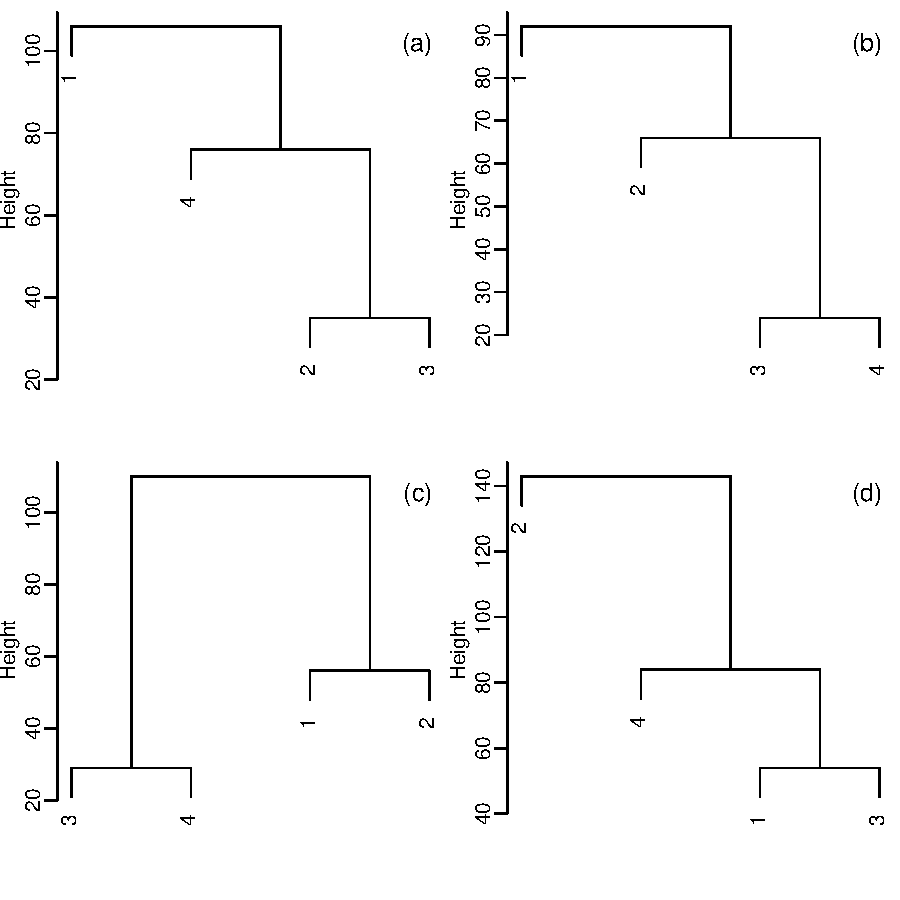
\includegraphics[width=\linewidth]{unsupervised-hclust.pdf}

\end{document}
